\documentclass[12pt, titlepage]{article}

\usepackage{fullpage}
\usepackage[round]{natbib}
\usepackage{multirow}
\usepackage{booktabs}
\usepackage{tabularx}
\usepackage{graphicx}
\usepackage{float}
\usepackage{hyperref}
\hypersetup{
    colorlinks,
    citecolor=black,
    filecolor=black,
    linkcolor=red,
    urlcolor=blue
}
\usepackage[round]{natbib}

\newcounter{acnum}
\newcommand{\actheacnum}{AC\theacnum}
\newcommand{\acref}[1]{AC\ref{#1}}

\newcounter{ucnum}
\newcommand{\uctheucnum}{UC\theucnum}
\newcommand{\uref}[1]{UC\ref{#1}}

\newcounter{mnum}
\newcommand{\mthemnum}{M\themnum}
\newcommand{\mref}[1]{M\ref{#1}}

\title{SE 3XA3: Module Guide \\ Scrabble}

\author{Team \#214, The Trifecta
		\\ Kanakabha Choudhri, Choudhrk
		\\ Lucia Cristiano, Cristial
		\\ Raymond Tu, Tur1
}

\date{March 13, 2020}

%\input{../../Comments}

\begin{document}

\maketitle

\pagenumbering{roman}
\tableofcontents
\listoftables
\listoffigures

\begin{table}[bp]
\caption{\bf Revision History}
\begin{tabularx}{\textwidth}{p{3cm}p{2cm}X}
\toprule {\bf Date} & {\bf Version} & {\bf Notes}\\
\midrule
13/2/20 & 1.0 & ---\\
\bottomrule
\end{tabularx}
\end{table}

\newpage

\pagenumbering{arabic}

\section{Introduction} %Raymond 

%Decomposing a system into modules is a commonly accepted approach to developing
%software.  A module is a work assignment for a programmer or programming
%team~\citep{ParnasEtAl1984}.  We advocate a decomposition
%based on the principle of information hiding~\citep{Parnas1972a}.  This
%principle supports design for change, because the ``secrets'' that each module
%hides represent likely future changes.  Design for change is valuable in SC,
%where modifications are frequent, especially during initial development as the
%solution space is explored.  
\subsection{Overview}

The Scrabble project is an implementation of the game Scrabble in python, with an ASCII based user interface on the command line terminal. The goal of the project is to take the original implementation on Github and improve on various aspects outlined in the SRS. The primary focus of these additional features is to implement a graphical user interface using the Tkinter library in python. This would make the game more accessible to users not familiar with use of the command line terminal, in an easily understood aesthetically pleasing format. Additionally, in the back-end modules will be re-implemented to allow for modularity and ease of maintainability for new features in the future. Overall, this would lead to better software design that is easier to maintain and update for the future. 

\subsection{Scope}

The scope of the project is based around the original Scrabble repository, any new features or functionality added is to make it closer to the original game. For example, there are several new modules added for background checks that are in line with the original rules of the game but omitted from the original Github implementation. The Tkinter library in Python will be the main tool used to create the GUI for Scrabble.

\subsection{Module Guide Purpose}
The purpose of this document, the Module Guide (MG) is to outline the modular structure of the system and allow any future contributors to easily identify parts of the program. New contributors will be able to refer to this document in the future to find relevant documentation for the modules they are working on. Additionally, the module guide will be helpful to check for consistency in the overall design of the game, the cohesion between modules and their coupling to ensure good software design. The module guide will outline how the modules in the back-end and front-end are broken up to have high cohesion and low coupling. Overall, the module guide will ensure developers and future contributors have good documentation to gain an understanding of the software, and ensure consistency between the relationships of the modules.

%Our design follows the rules layed out by \citet{ParnasEtAl1984}, as follows:
%\begin{itemize}
%\item System details that are likely to change independently should be the
%  secrets of separate modules.
%\item Each data structure is used in only one module.
%\item Any other program that requires information stored in a module's data
%  structures must obtain it by calling access programs belonging to that module.
%\end{itemize}

%After completing the first stage of the design, the Software Requirements
%Specification (SRS), the Module Guide (MG) is developed~\citep{ParnasEtAl1984}. %The MG
%specifies the modular structure of the system and is intended to allow both
%designers and maintainers to easily identify the parts of the software.  The
%potential readers of this document are as follows:

%\begin{itemize}
%\item New project members: This document can be a guide for a new project member
%  to easily understand the overall structure and quickly find the
%  relevant modules they are searching for.
%\item Maintainers: The hierarchical structure of the module guide improves the
%  maintainers' understanding when they need to make changes to the system. It is
%  important for a maintainer to update the relevant sections of the document
%  after changes have been made.
%\item Designers: Once the module guide has been written, it can be used to
%  check for consistency, feasibility and flexibility. Designers can verify the
%  system in various ways, such as consistency among modules, feasibility of the
%  decomposition, and flexibility of the design.
%\end{itemize}

The rest of the document is organized as follows. Section
\ref{SecChange} lists the anticipated and unlikely changes of the software
requirements. Section \ref{SecMH} summarizes the module decomposition that
was constructed according to the likely changes. Section \ref{SecConnection}
specifies the connections between the software requirements and the
modules. Section \ref{SecMD} gives a detailed description of the
modules. Section \ref{SecTM} includes two traceability matrices. One checks
the completeness of the design against the requirements provided in the SRS. The
other shows the relation between anticipated changes and the modules. Section
\ref{SecUse} describes the use relation between modules.

\section{Anticipated and Unlikely Changes} \label{SecChange} %Raymond

This section lists possible changes to the system. According to the likeliness
of the change, the possible changes are classified into two
categories. Anticipated changes are listed in Section \ref{SecAchange}, and
unlikely changes are listed in Section \ref{SecUchange}. Anticipated changes are feasible changes that will be implemented in the future, while unlikely changes are those that may improve the quality of the user experience but are not likely to be implemented.

\subsection{Anticipated Changes} \label{SecAchange}

%Anticipated changes are the source of the information that is to be hidden
%inside the modules. Ideally, changing one of the anticipated changes will only
%require changing the one module that hides the associated decision. The approach
%adapted here is called design for
%change.

\begin{description}
\item [\refstepcounter{acnum} \actheacnum \label{acSkipTurn}:] Implementation of a Skip Turn button. This would prevent deadlock in the game if a player is unable to make a move. 
\item [\refstepcounter{acnum} \actheacnum \label{acExchangeTile}:] Implementation of an Exchange Tiles button. This would help prevent deadlock if available tiles do not create a word that can be placed.
\item [\refstepcounter{acnum} \actheacnum \label{acScoreboard}:] Scoreboard at the end of a match. Display player total score and who won at the end of a match. 
\item [\refstepcounter{acnum} \actheacnum \label{acGUI}:] Improved user interface, more adjustable window resolution and default size. Make the interface more friendly to different monitor sizes, and more readable text/font sizes.
\end{description}

\subsection{Unlikely Changes} \label{SecUchange}

%The module design should be as general as possible. However, a general system is
%more complex. Sometimes this complexity is not necessary. Fixing some design
%decisions at the system architecture stage can simplify the software design. If
%these decision should later need to be changed, then many parts of the design
%will potentially need to be modified. Hence, it is not intended that these
%decisions will be changed.

\begin{description}
\item [\refstepcounter{ucnum} \uctheucnum \label{ucIO}:] Input/Output devices. It is possible that the input may be changed from the default keyboard and mouse to other forms such as a touch screen, but given the scope of the project this is unlikely to occur.
\item [\refstepcounter{ucnum} \uctheucnum \label{ucEnviro}:] Different environments/platforms. It is possible for portability that additional environments/platforms other than Windows OS are supported, for example the Scrabble game as a mobile application on Android of Apple OS, but given the scope of project this is unlikely.
\item [\refstepcounter{ucnum} \uctheucnum \label{ucNumPlay}:] Different numbers of players. It is possible to enhance the user experience by allowing more than 2 players to play at once and balance the game accordingly with varying types of scoring and number of tiles in the bag to adjust game length. However, given the scope and timeframe of the project this is unlikely to occur.
\item [\refstepcounter{ucnum} \uctheucnum \label{ucSP}:] Singleplayer options. It would be possible to create a singleplayer option where the player faces the computer designed with machine learning. However, this is outside of the scope of the project and is unlikely to be implemented.
\end{description}

\section{Module Hierarchy} \label{SecMH} %Raymond

This section provides an overview of the module design. Modules are summarized
in a hierarchy decomposed by secrets in Table \ref{TblMH}. The modules listed
below, which are leaves in the hierarchy tree, are the modules that will
actually be implemented.

\begin{description}
\item [\refstepcounter{mnum} \mthemnum \label{mHHGW}:] Game Window %Hardware-Hiding Module
\item [\refstepcounter{mnum} \mthemnum \label{mBHGB}:] Gameboard Boolean Checks % Behaviour Hiding
\item [\refstepcounter{mnum} \mthemnum \label{mBHET}:] End Turn Boolean Checks % Behaviour Hiding
\item [\refstepcounter{mnum} \mthemnum \label{mBHVW}:] Valid Word Boolean Checks % Behaviour Hiding
\item [\refstepcounter{mnum} \mthemnum \label{mBHGV}:] Game View % Behaviour Hiding
\item [\refstepcounter{mnum} \mthemnum \label{mSDBO}:] Board % Software Decision
\item [\refstepcounter{mnum} \mthemnum \label{mSDP}:] Player % Software Decision
\item [\refstepcounter{mnum} \mthemnum \label{mSDR}:] Rack % Software Decision
\item [\refstepcounter{mnum} \mthemnum \label{mSDT}:] Tiles % Software Decision
\item [\refstepcounter{mnum} \mthemnum \label{mSDB}:] Bag % Software Decision
\end{description}


\begin{table}[h!]
\centering
\begin{tabular}{p{0.3\textwidth} p{0.6\textwidth}}
\toprule
\textbf{Level 1} & \textbf{Level 2}\\
\midrule

{Hardware-Hiding Module} & Game Window \\
\midrule

\multirow{2}{0.3\textwidth}{Behaviour-Hiding Module} & Game View\\
& End Turn Boolean Checks\\

\midrule

\multirow{7}{0.3\textwidth}{Software Decision Module} & Bag\\
& Board\\
& Player\\
& Rack\\
& Tiles\\
& Valid Word Boolean Checks\\
& Gameboard Boolean Checks\\
\bottomrule

\end{tabular}
\caption{Module Hierarchy}
\label{TblMH}
\end{table}

\newpage 

\section{Connection Between Requirements and Design} %Kanak \label{SecConnection}

\begin{table}[htp]
\centering
\begin{tabular}{|l|l|}
\hline
\textbf{Module} & \textbf{Requirement Module Meets}                                                                                                                   \\ \hline
Tile            & FR10, MS1, MS2, MS3, LR1                                                                                                                            \\ \hline
Bag             & FR5, MS1, MS2, MS3, LR1                                                                                                                             \\ \hline
Rack            & FR11, MS1, MS2, MS3, LR1                                                                                                                            \\ \hline
Player          & FR4, MS1, MS2, MS3, LR1                                                                                                                             \\ \hline
Board           & FR2, MS1, MS2, MS3, LR1                                                                                                                             \\ \hline
EndTurn         & FR10, MS1, MS2, MS3, LR1                                                                                                                            \\ \hline
WordChecks      & FR6, MS1, MS2, MS3, CR1, LR1                                                                                                                        \\ \hline
BoardChecks     & FR6, FR8, FR9, MS1, MS2, MS3, LR1                                                                                                                   \\ \hline
MainGame        & \begin{tabular}[c]{@{}l@{}}FR2, FR4, FR7, FR8, FR10, FR12, \\ LF1, UH1, UH2, UH3, UH4, UH5, UH7,\\  PR1, PR2, OE1, OE2, CR1, LR1, HSR1\end{tabular} \\ \hline
\end{tabular}
\caption{ Requirements and Design Connection}
\label{TblRDC}
\end{table}

\section{Module Decomposition} \label{SecMD} %Lucia

The purpose of having modules is to decompose the system into manageable pieces that can be more easily developed than a monolithic piece of software. The way modules are decomposed is based around the principle of information hiding, which states that each module has one secret that is hidden from the other modules. These secrets are parts of the implementation that are likely to change. Each module also has a service which is the functionality that the module provides without describing the implementation of these services. For each of the modules given in the hierarchy their secret and service is listed as well as how the module will be implemented.

% Modules are decomposed according to the principle of ``information hiding''
% proposed by \citet{ParnasEtAl1984}. The \emph{Secrets} field in a module
% decomposition is a brief statement of the design decision hidden by the
% module. The \emph{Services} field specifies \emph{what} the module will do
% without documenting \emph{how} to do it. For each module, a suggestion for the implementing software is given under the \emph{Implemented By} title. If the entry is \emph{OS}, this means that the module is provided by the operating system or by standard programming language libraries.  Also indicate if the module will be implemented specifically for the software.

% Only the leaf modules in the
% hierarchy have to be implemented. If a dash (\emph{--}) is shown, this means
% that the module is not a leaf and will not have to be implemented. Whether or not this module is implemented depends on the programming language selected.

\subsection{Hardware Hiding Modules - Game Window (\mref{mHHGW})} 
\begin{description}
\item[Secrets:]The data structures and algorithms used to handle virtual input and output, for example the screen, keyboard and mouse.
\item[Services:]Serves as a virtual hardware for the screen, keyboard, mouse used by the rest of the system to accept input and display output to the screen. This module provides the interface between the hardware and the
software.
\item[Implemented By:] OS
\end{description}

\subsection{Behaviour-Hiding Module}
\begin{description}
\item[Secrets:]The contents of the required behaviours of the player and the game board interface.
\item[Services:]Includes programs that provide externally visible behaviour of
  the game board as outlined in the software requirements specification (SRS)
  document. These modules serve as a middle layer that provides communication layer between the hardware-hiding module and the software decision modules. The programs in this module will need to change if there are changes in the SRS as these modules deal with the implementation of the functional requirements.
\item[Implemented By:] Scrabble Project
\end{description}

\subsubsection{End Turn Boolean Checks (\mref{mBHET})}
\begin{description}
\item[Secrets:]The logic for when a move is completed by a player.
\item[Services:] Provides the behaviour necessary for updating the interface based on changes in data once the player has made a move.
\item[Implemented By:] Scrabble Project
\end{description}

\subsubsection{Game View (\mref{mBHGV})}
\begin{description}
\item[Secrets:]The interface of the game that the player interacts with.
\item[Services:]Displays the game board, input boxes and buttons necessary for the player to interact with the game.
\item[Implemented By:] Scrabble Project
\end{description}




\subsection{Software Decision Module}
\begin{description}
\item[Secrets:] The design decision based on mathematical theorems, physical
  facts, or programming considerations. The secrets of this module are
  \emph{not} described in the SRS.
\item[Services:] Includes data structure and algorithms used in the system that
  do not provide direct interaction with the user. Changes to these modules are more likely to be motivated by a desire to improve performance than by externally imposed changes.
\item[Implemented By:] --
\end{description}

\subsubsection{Gameboard Boolean Checks (\mref{mBHGB})}
\begin{description}
\item[Secrets:]The algorithms dealing with the correct placement of words on the board.
\item[Services:]Provides the behaviour associated with ensuring that a word is correctly placed on the board. 
\item[Implemented By:] Scrabble Project
\end{description}

\subsubsection{Valid Word Boolean Checks (\mref{mBHVW})}
\begin{description}
\item[Secrets:]The algorithms to determine if a valid word is entered by the player
\item[Services:] Provides the behaviour necessary for ensuring that only valid words are used in the game.
\item[Implemented By:] Scrabble Project
\end{description}

\subsubsection{Board (\mref{mSDBO})}
\begin{description}
\item[Secrets:] The data structure that represent the Scrabble game board.
\item[Services:] Includes data structure, setters and getters used to model the board of a game of Scrabble. Used by checks to ensure correct placement of words.
\item[Implemented By:] Scrabble Project
\end{description}

\subsubsection{Player (\mref{mSDP})}
\begin{description}
\item[Secrets:] The data structure that represents a player participating in a Scrabble game.
\item[Services:] Includes data structure, setters and getters used to model the data associated with a player, such as score and rack of tiles.
\item[Implemented By:] Scrabble Project
\end{description}

\subsubsection{Rack (\mref{mSDR})}
\begin{description}
\item[Secrets:] The data structure that represents a rack of tiles in a Scrabble game.
\item[Services:] Includes data structure, setters and getters used to model a generic rack of game tiles. 
\item[Implemented By:] Scrabble Project
\end{description}

\subsubsection{Tiles (\mref{mSDT})}
\begin{description}
\item[Secrets:] The data structure that represents a tile in a Scrabble game.
\item[Services:] Includes data structure, setters and getters used to model the tile such as score and letter.
\item[Implemented By:] Scrabble Project
\end{description}

\subsubsection{Bag (\mref{mSDB})}
\begin{description}
\item[Secrets:] The data structure that represent the bag of tiles.
\item[Services:] Includes data structure, setters and getters used to model the bag aspect of a game of Scrabble.
\item[Implemented By:] Scrabble Project
\end{description}


\section{Traceability Matrix} \label{SecTM} % Lucia

This section shows two traceability matrices: between the modules and the
requirements and between the modules and the anticipated changes. Some functional requirements, namely FR1 and FR3 have been deemed obsolete based on feedback from teaching assistants and review of the requirements by the team.
 
\begin{table}[H]
\centering
\begin{tabular}{p{0.2\textwidth} p{0.6\textwidth}}
\toprule
\textbf{Req.} & \textbf{Modules}\\
\midrule
FR1 & Obsolete \\
FR2 & \mref{mHHGW}, \mref{mBHGV}, \mref{mSDBO}\\
FR3 & Obsolete \\
FR4 & \mref{mHHGW}, \mref{mBHGV}\\
FR5 & \mref{mHHGW}, \mref{mBHGV}, \mref{mSDR}, \mref{mSDT}\\
FR6 & \mref{mHHGW}, \mref{mBHGV}, \mref{mBHVW}\\
FR7 & \mref{mHHGW}, \mref{mBHGV}\\
FR8 & \mref{mHHGW}, \mref{mBHGV}, \mref{mBHGB}\\
FR9 & \mref{mHHGW}, \mref{mBHGV}, \mref{mBHGB}, \mref{mSDBO}\\
FR10 & \mref{mHHGW}, \mref{mBHGV}, \mref{mSDT}\\
FR11 & \mref{mHHGW}, \mref{mBHGV}\\
FR12 & \mref{mHHGW}, \mref{mBHGV}, \mref{mBHET}, \mref{mSDB}\\
\bottomrule
\end{tabular}
\caption{Trace Between Requirements and Modules}
\label{TblRT}
\end{table}

\begin{table}[H]
\centering
\begin{tabular}{p{0.2\textwidth} p{0.6\textwidth}}
\toprule
\textbf{AC} & \textbf{Modules}\\
\midrule
\acref{acSkipTurn} & \mref{mBHGV}\\ %game view
\acref{acExchangeTile} & \mref{mBHGV}\\
& \mref{mBHET}\\ %exchange tile 
\acref{acScoreboard} & \mref{mBHGV}\\
\acref{acGUI} & \mref{mBHGV}\\
& \mref{mHHGW}\\
\bottomrule
\end{tabular}
\caption{Trace Between Anticipated Changes and Modules}
\label{TblACT}
\end{table}

\section{Use Hierarchy Between Modules} \label{Module Hierarchy} %Kanak

\begin{figure}[H]
\centering
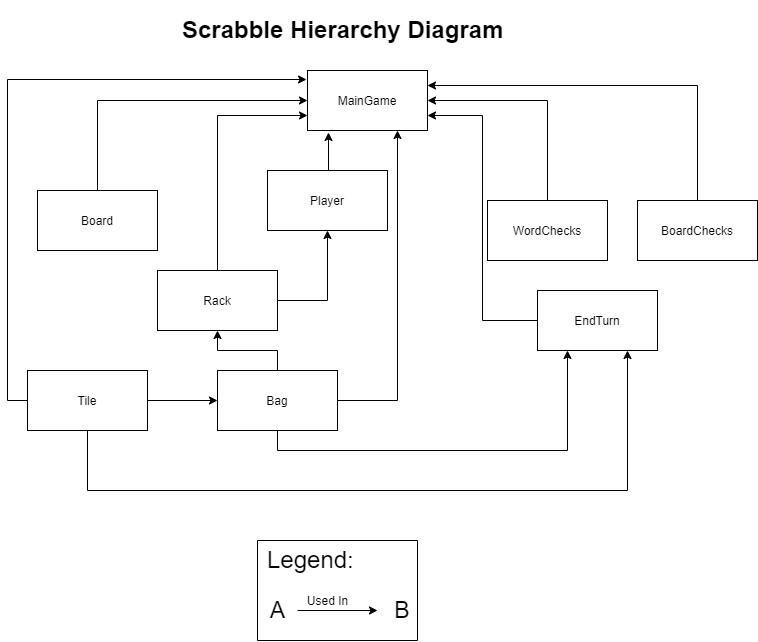
\includegraphics[width=0.7\textwidth]{mg_section7.png}
\caption{Use hierarchy among modules}
\label{FigUH}
\end{figure}

%\section*{References}

% \bibliographystyle {plainnat}
% \bibliography {MG}

\end{document}